\section{Introduction}

Le syst\`{e}me consid\'{e}r\'{e} est un satellite de masse fix\'{e} $m$ lib\'{e}r\'{e}
par une fus\'{e}e dans le plan de l'\'{e}quateur; l'orbite initiale du satellite est
une ellipse de forte excentricit\'{e}, voir figure~\ref{figtransfert}. L'objectif de ce travail est de r\'{e}aliser
le transfert en temps minimal de cette orbite elliptique \`{a} une orbite circulaire 
g\'{e}ostationnaire. 

\begin{figure}[ht!]
\centering
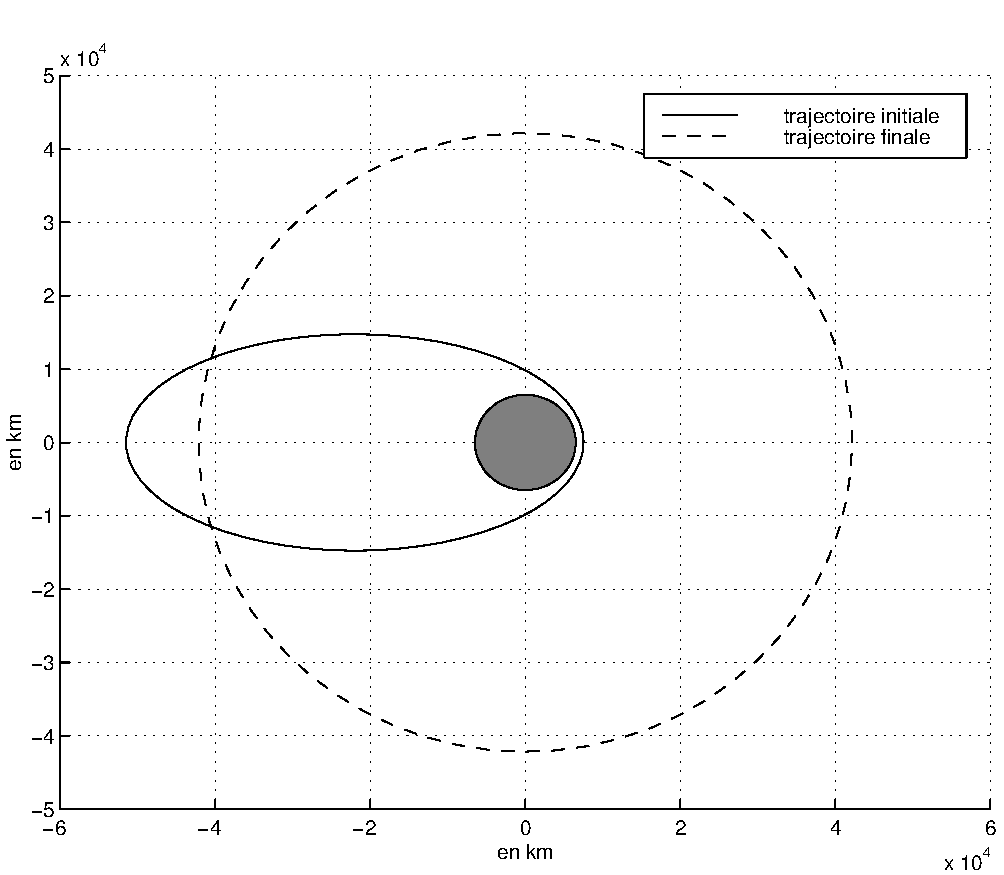
\includegraphics[height=5.0cm]{./fig1transfert}
\caption{\label{figtransfert}Transfert orbital 2D.}
\end{figure}

\section{R\'esolution du probl\`eme en temps minimal}

Consid\'erons le probl\`eme de transfert orbital \`a temps minimal suivant~:
\leqnomode
\begin{equation}\label{eq:transfert_temps_min}
    \tagProblem
        \left\{
            \begin{array}{l}
                \displaystyle J(u(\cdot), t_f) = t_f \longrightarrow \min                                \\[1.0em]
                \displaystyle \dot{x}_1(t) = x_3(t), \\[0.5em]
                \displaystyle \dot{x}_2(t) = x_4(t), \\[0.5em]
                \displaystyle \dot{x}_3(t) = -\frac{\mu\, x_1(t)}{{r(t)}^3} + u_1(t), \\[0.5em]
                \displaystyle \dot{x}_4(t) = -\frac{\mu\, x_2(t)}{{r(t)}^3} + u_2(t),
                \quad \norme{u(t)} \le \gamma_\mathrm{max}, 
                \quad t \in \intervalleff{0}{t_f} \text{ p.p.}, \quad u(t) \coloneqq(u_1(t),u_2(t)),     \\[1.0em]
                \displaystyle x_1(0) = x_{0,1},   \quad x_2(0) = x_{0,2},  \quad x_3(0) = x_{0,3}, \quad x_4(0) = x_{0,4},  \\[1.0em]
                \displaystyle r(t_f)^2 = r_f^2, \quad
                \displaystyle x_3(t_f) = - \sqrt{\frac{\mu}{r_f^3}}\, x_2(t_f), \quad
                \displaystyle x_4(t_f) = \sqrt{\frac{\mu}{r_f^3}}\, x_1(t_f),
            \end{array} 
        \right.
\end{equation}
\reqnomode
avec $r(t) \coloneqq \sqrt{x_1(t)^2 + x_2(t)^2}$. Les unit\'es choisies sont le kilom\`etre pour les distances et l'heure pour les temps, \cf
table \ref{table:transfert_temps_min_data}.

\begin{table}[ht!]
    \centering
    \begin{tabular}{lll}
        \medhrule
        Param\`etre                                & Valeur & Unit\'e   \\
        \bighrule
        $\mu$                   & $5.1658620912\times10^{12}$  & km$^3$ h$^{-2}$ \\
        $r_f$                   & $42165$                           & km \\
        $\gamma_\mathrm{max}$   & $388.8$                           & km h$^{-2}$ \\
        \medhrule
        \\
    \end{tabular}
    \caption{Unit\'e et valeurs des param\`etres constants. Cette valeur de $\gamma_\mathrm{max}$ correspond \`a une acc\'el\'eration de 60N et \`a
    une masse de 2000kg, \cf $\gamma_\mathrm{max} = \frac{F_\mathrm{max}}{m} = \frac{60 \times 3600^2}{2000 \times 10^3} = 388.8$.}
    \label{table:transfert_temps_min_data}
\end{table}

Le pseudo-hamiltonien est donn\'e par : 
\[
    H(x,p,u) = x_3\, p_1 + x_4\, p_2 + \left(u_1 - \frac{\mu\, x_1}{\norme{r}^3}\right) p_3 + \left(u_2 - \frac{\mu\, x_2}{\norme{r}^3}\right) p_4.
\]
On consid\`ere le cas normal et on fixe $p^0=-1$.
La condition de maximisation nous donne comme loi de commande :
\[
    u(t) = \usol(z(t)) \coloneqq \frac{\gamma_\mathrm{max}}{\sqrt{p_3(t)^2+p_4(t)^2}} \left( p_3(t) , p_4(t) \right).
\]
Le temps final \'etant libre, on a la condition au temps final $H(x(t_f), p(t_f), u(t_f)) = -p^0$ et
puisque le point terminal sur l'orbite final n'est pas enti\`erement fix\'e, le PMP nous donne la condition de transversalit\'e en $t_f$ 
suivante :
\[
    x_2(t_f) \left( p_1(t_f) + \sqrt{\frac{\mu}{r_f^3}}\, p_4(t_f) \right) = x_1(t_f) \left( p_2(t_f) - \sqrt{\frac{\mu}{r_f^3}}\, p_3(t_f) \right).
\]
En introduisant $\alpha \coloneqq \sqrt{\frac{\mu}{r_f^3}}$, la fonction de tir multiple s'\'ecrit :
\begin{equation*}
    \begin{array}{rlll}
        S \colon    & \R^5          & \longrightarrow   & \R^5 \\
        & (p_0, t_f)      & \longmapsto       &
        \begin{bmatrix}
            \sqrt{x_1(t_f, z_0)^2 + x_2(t_f, z_0)^2} - r_f \\[0.5em]
            x_3(t_f, z_0) + \alpha\, x_2(t_f, z_0) \\[0.5em]
            x_4(t_f, z_0) - \alpha\, x_1(t_f, z_0) \\[0.5em]
            x_2(t_f, z_0) \left( p_1(t_f, z_0) + \alpha\, p_4(t_f, z_0) \right) - x_1(t_f, z_0) \left( p_2(t_f, z_0) - \alpha\, p_3(t_f, z_0) \right) \\[0.5em]
            H(z(t_f, z_0), \usol(z(t_f, z_0))) + p^0
        \end{bmatrix},
    \end{array}
\end{equation*}
o\`u $z_0 \coloneqq (x_0, p_0)$, $x_0 \coloneqq (x_{0,1}, x_{0,2}, x_{0,3}, x_{0,4})$, $z(\cdot, z_0) \coloneqq (x(\cdot, z_0), p(\cdot, z_0))$ et
$x \coloneqq (x_1, x_2, x_3, x_4)$, $p\coloneqq (p_1, p_2, p_3, p_4)$.

\begin{myremark}
    Pour la r\'esolution num\'erique, il est pr\'ef\'erable de remplacer l'\'equation $r(t_f)^2 = r_f^2$ par $r(t_f) = r_f$.
\end{myremark}

\begin{myExercice} Se rendre dans le r\'epertoire \cmd{TP4\_transfert\_orbital\_temps\_min}.
    \begin{enumerate}
        \item Compl\'eter seulement \cmd{sfun} dans \cmd{sfun.f90}.
        \item Compiler le probl\`eme.
        \item Jeter un \oe il au script \matlab\ \cmd{main41.m} puis l'ex\'ecuter.
    \end{enumerate}
\end{myExercice}



